\section{Proposed ChatBot}
% 
\subsection{DataModel}
It seems obvious that browsing our 2,249,053 lines-long corpus for each query wasn't such a great idea, that's why we stored the data in a re-usable DBMS.
\subsubsection{Chosen technology}
We considered 2 options : a traditional DBMS such as MySQL or a graph-oriented DBMS. We finally chose to use a graph model for several reasons :
\begin{itemize}
\item For a corpus such as ours, with a lot of n-1..n relations, a graph allows the user to build queries who look like \say{paths}. It is both more efficient (no table join, less computation time) and more natural for the user.
\item Graph-base DBMS doesn't require a rigid schema, which means that we can create new kind of entities and relationships \say{on the go}.
\item It supports indexes and unique constraints 
\item Most of the graph-based systems implements useful algorithms such as the shortest path between two nodes. 
\end{itemize}
Regarding the technology, Neo4j\footnote{http://neo4j.com/} was chosen in regards of those facts :\\
\begin{itemize}
\item One of us (Mael) was already working with it for his MasterArbeit and was familiar with the language used to build Neo4j queries (Cypher).
\item Neo4j is cross-platform
\item The community is strong, there're even french groups
\item The technology is mature, 15 years old and currently running version 2.2
\item It provides a nice browser interface
\end{itemize}
\subsubsection{Structure}
Here, we will describe the actual structure of the corpus-graph. Remember that it isn't rigid so it might vary over the project's progress.\\
Other nodes and relationships exist in our database but are used for other purposes such as the history of the conversation or some probabilities (see section \ref{sssec:v_stype}).\\
Basically we can say that in our case, one vertex equals one XML tag. Instead of listing all the vertexes and the edges, we provide here an example based on a dialogue from the movie\footnote{12 Monkeys on IMDB : http://www.imdb.com/title/tt0114746/} \say{12 Monkeys}.
\lstinputlisting[language=XML,caption=XML extract,label={code:extr}]{graphExample.xml}
\begin{figure}[!h]
\begin{center}
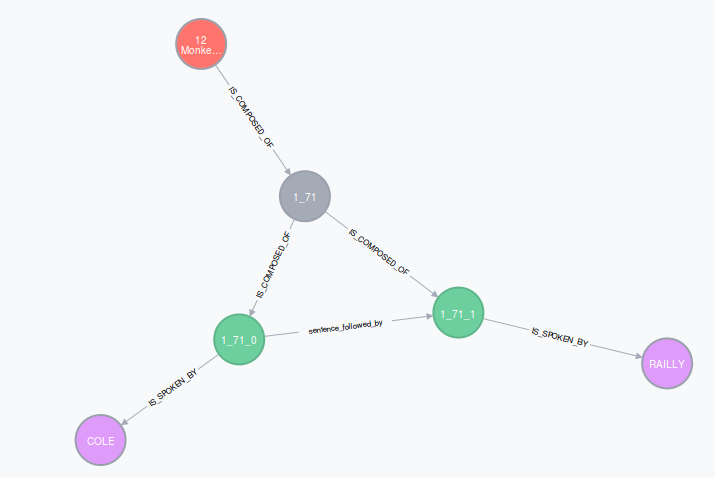
\includegraphics[width=0.6\textwidth]{graph171.png}
\end{center}
\caption{Neo4j modelisation}
\label{fig:neoExtr}
\end{figure}
With the above example we see that, just like in the XML (Code \ref{code:extr}), a \textbf{Movie} (pink) \textit{IS\_COMPOSED\_OF} \textbf{Dialogues} (gray, only one displayed here) which \textit{IS\_COMPOSED\_OF} several \textbf{Sentences} (green). Each sentence \textit{IS\_SPOKEN\_BY} a \textbf{Character} (purple).\\
The labels of the dialogues and sentences are an aggregation of the id fields of their parents :
\begin{center}Sentence\_Node\_id = idMovie\_idDialogue\_idSentence \end{center}
Now that we have represented the corpus as a graph, we can start to work with the NLP technology. Each sentence his processed and \dots \\
\textbf{LEO, BLABLA A PROPOS DU DECOUPAGE EN TOKEN ET LES SENTENCESTYPES, REF A FIG.15}
\begin{figure}[!h]
\begin{center}
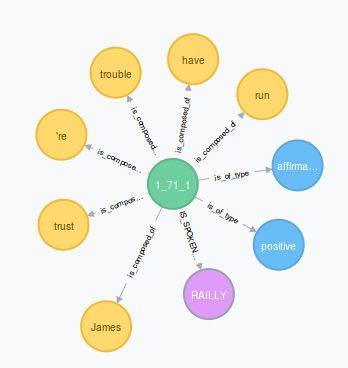
\includegraphics[width=0.5\textwidth]{graph1711.png}
\end{center}
\caption{Sentence details}
\label{fig:sent}
\end{figure}
% 
\subsection{User Interface}
\subsubsection{Chosen technology}
% 
\subsection{Anna's answers}
\subsubsection{Version 1 : Random answers}
\label{sssec:v_rand}

\subsubsection{Version 2 : Determined SentenceType}
\label{sssec:v_stype}

\subsubsection{Version 3 : Determined movie genre}
\label{sssec:v_genre}